\chapter{Généralités UML et Conception du système}
\label{chap:conception}

\section{Le langage UML}
\label{sec:langage_uml}

\subsection{Définition}
\label{subsec:definition_uml}

UML, ou \textit{Unified Modeling Language}, se définit comme un langage de modélisation graphique et textuel destiné à comprendre et décrire des besoins, spécifier, concevoir des solutions et communiquer des points de vue. Il ne s’agit pas d’une simple notation graphique, car les concepts transmis par un diagramme ont une sémantique précise et sont porteurs de sens au même titre que les mots d’un langage.

UML permet de visualiser, spécifier, construire et documenter les éléments d’un système logiciel \cite{omg_uml_spec}. Il est aussi utilisé pour modéliser la structure, le comportement et l’architecture des applications, ainsi que les processus métier et les structures de données \cite{omg_uml}. Dans notre projet, UML est utilisé pour exprimer les besoins et décrire la conception de notre application de gestion de courrier.

\subsection{Caractéristiques d’UML}
\label{subsec:caracteristiques_uml}

Dans le cadre de la modélisation d’une application informatique, UML possède plusieurs caractéristiques importantes.

Tout d’abord, UML n’est pas une méthode ou un processus. Il ne définit pas l’enchaînement complet des activités de développement, mais il fournit un langage permettant de représenter les différents aspects d’un système. Le choix de la démarche reste donc indépendant du langage UML.

Ensuite, UML est un langage semi-formel. Il repose sur des concepts de modélisation ayant une signification précise. Cela permet de réduire les ambiguïtés et de faciliter la compréhension entre les membres d’une équipe de projet.

UML possède aussi une représentation graphique standardisée. Cette notation commune permet aux analystes, développeurs et autres intervenants de lire les mêmes diagrammes avec une compréhension proche.

Enfin, UML offre plusieurs vues complémentaires d’un système. Chaque diagramme présente une partie différente : les besoins, les acteurs, les échanges, les classes, les états ou encore l’architecture technique. Cette séparation aide à mieux maîtriser la complexité d’un système.

\subsection{Les points forts et faibles d’UML}
\label{subsec:points_forts_faibles_uml}

\subsubsection{Les points forts d’UML}
\label{subsubsec:points_forts_uml}

UML est un langage formel et normalisé. Il permet de gagner en précision, d’encourager l’utilisation d’outils de modélisation et de garder une documentation claire du système. Son caractère visuel facilite aussi la communication entre les différents acteurs du projet.

UML est également un bon support de communication. Il cadre l’analyse et facilite la compréhension de représentations parfois abstraites. Grâce à ses différents diagrammes, il devient plus simple d’expliquer le fonctionnement général d’une application avant de passer au développement.

Par rapport à Merise, UML est plus adapté à la conception orientée objet. Il permet de représenter à la fois les données, les traitements, les interactions et le comportement du système. Merise reste utile pour les systèmes fortement centrés sur les données, mais UML est souvent plus souple pour les applications web modernes, où les objets métier, les interfaces et les échanges évoluent ensemble.

\subsubsection{Les points faibles d’UML}
\label{subsubsec:points_faibles_uml}

La mise en pratique d’UML demande un apprentissage. Il faut comprendre le rôle de chaque diagramme et savoir lequel utiliser selon le besoin. Si tous les diagrammes sont utilisés sans nécessité, la conception peut devenir lourde.

UML ne remplace pas non plus une méthode de gestion de projet. Il permet de modéliser le système, mais il ne dit pas exactement comment organiser toutes les étapes du développement. Il doit donc être utilisé avec une démarche claire, en choisissant seulement les diagrammes utiles pour le projet.

\section{Conception du système}
\label{sec:conception_systeme}

Dans cette section, nous présentons les différents diagrammes réalisés pour la conception de notre application.

\subsection{Étude préliminaire}
\label{subsec:etude_preliminaire}

Avant de présenter les différents diagrammes de conception, nous réalisons une étude préliminaire afin d’identifier les acteurs qui interagissent avec le système ainsi que les principales fonctionnalités offertes par l’application.

\subsubsection{Identification des acteurs}
\label{subsubsec:identification_acteurs}

Les principaux acteurs du système sont :

\begin{itemize}
    \item \textbf{Agent} : consulte les courriers qui lui sont destinés et répond aux courriers nécessitant une réponse.
    \item \textbf{Secrétaire} : consulte, répond et transmet les courriers liés à son organe.
    \item \textbf{Secrétaire générale} : crée et suit les courriers reçus au niveau de l’établissement.
    \item \textbf{Chef d’organe} : valide, transmet et suit les courriers de son organe.
    \item \textbf{Chef général} : supervise le traitement global des courriers et valide les courriers au niveau de l’établissement.
    \item \textbf{Administrateur} : gère les utilisateurs, le référentiel et la configuration du système.
\end{itemize}

\subsubsection{Identification des fonctionnalités}
\label{subsubsec:identification_fonctionnalites}

Les principales fonctionnalités du système sont :

\begin{itemize}
    \item l’authentification des utilisateurs ;
    \item la gestion des utilisateurs ;
    \item la création des courriers ;
    \item la consultation des courriers ;
    \item la transmission des courriers ;
    \item la validation des courriers ;
    \item la réponse aux courriers ;
    \item la recherche des courriers ;
    \item l’archivage des courriers ;
    \item l’administration du référentiel et de la configuration.
\end{itemize}
\subsection{Diagramme de classes}
\label{subsec:diagramme_classes}

\begin{figure}[h]
    \centering
    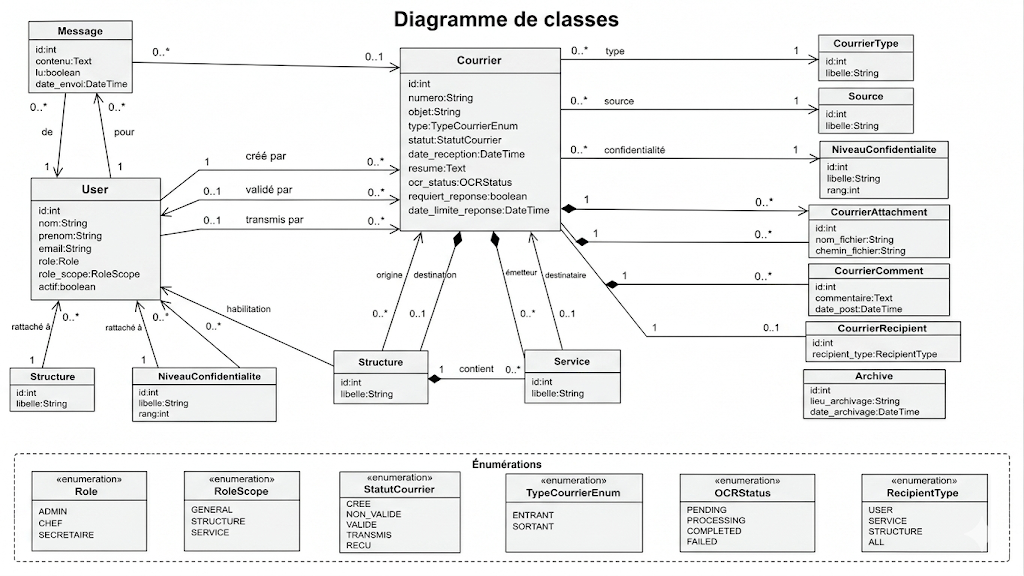
\includegraphics[width=\textwidth,height=0.85\textheight,keepaspectratio]{diagrams/classD/classD.png}
    \caption{Diagramme de classes de l’application}
    \label{fig:diagramme_classes}
\end{figure}

\subsection{Diagrammes de cas d’utilisation}
\label{subsec:diagrammes_cas_utilisation}

\subsubsection{Diagramme de cas d’utilisation global}
\label{subsubsec:cas_utilisation_global}

\begin{figure}[H]
    \centering
    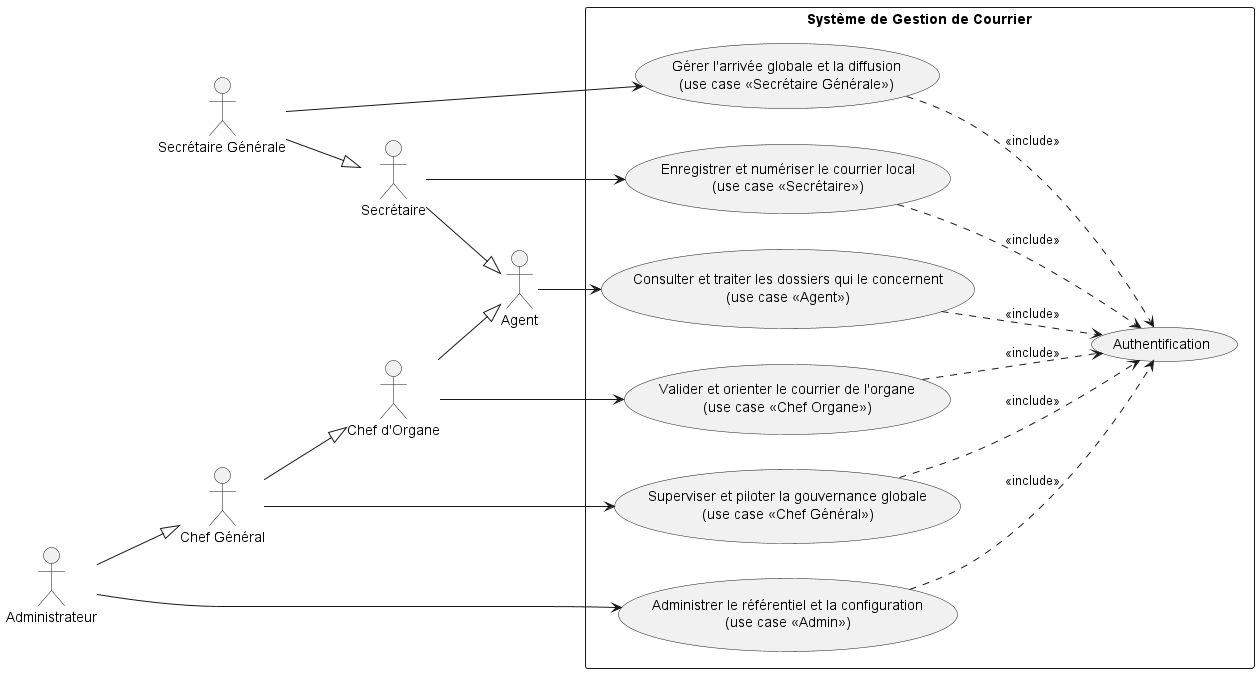
\includegraphics[width=14cm]{out/diagrams/usecases/puml/usecase_global/usecase_global.png}
    \caption{Diagramme de cas d’utilisation global}
    \label{fig:cas_utilisation_global}
\end{figure}

\subsubsection{Diagramme de cas d’utilisation de l’administrateur}
\label{subsubsec:cas_utilisation_admin}

\begin{figure}[H]
    \centering
    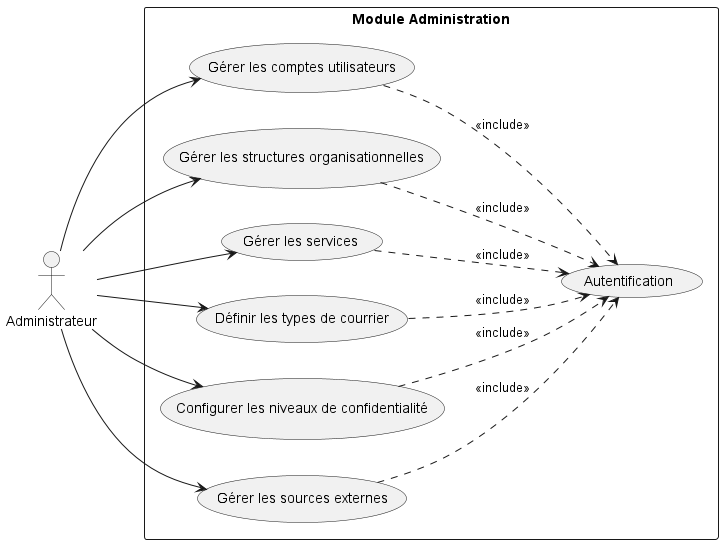
\includegraphics[width=14cm]{out/diagrams/usecases/puml/usecase_admin/usecase_admin.png}
    \caption{Diagramme de cas d’utilisation de l’administrateur}
    \label{fig:cas_utilisation_admin}
\end{figure}

\subsubsection{Diagramme de cas d’utilisation du chef général}
\label{subsubsec:cas_utilisation_chef_general}

\begin{figure}[H]
    \centering
    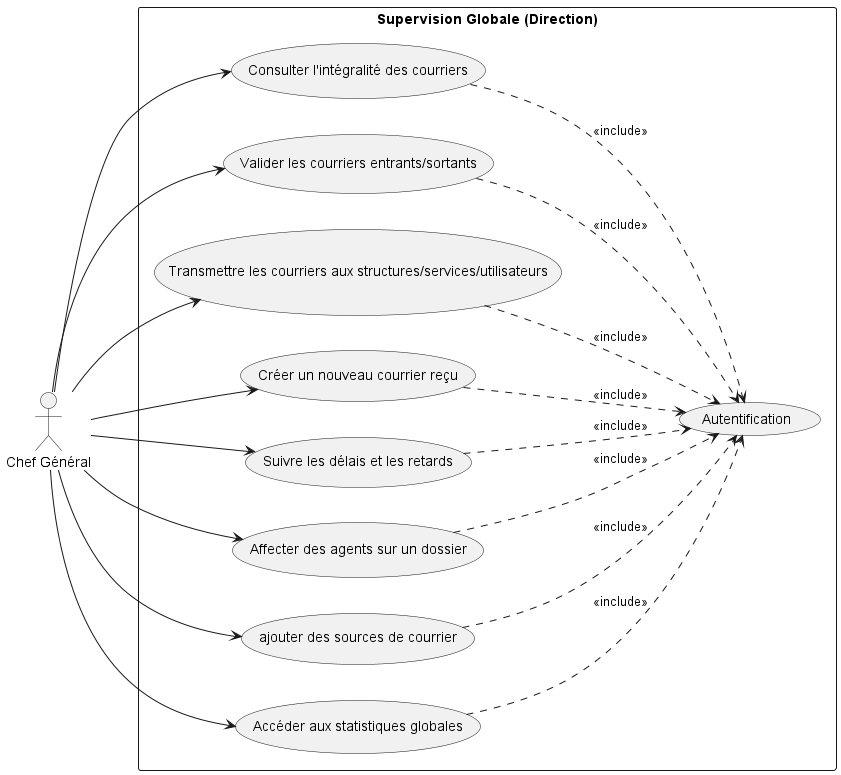
\includegraphics[width=14cm]{out/diagrams/usecases/puml/usecase_chef_general/usecase_chef_general.png}
    \caption{Diagramme de cas d’utilisation du chef général}
    \label{fig:cas_utilisation_chef_general}
\end{figure}

\subsubsection{Diagramme de cas d’utilisation de la secrétaire générale}
\label{subsubsec:cas_utilisation_secretaire_generale}

\begin{figure}[H]
    \centering
    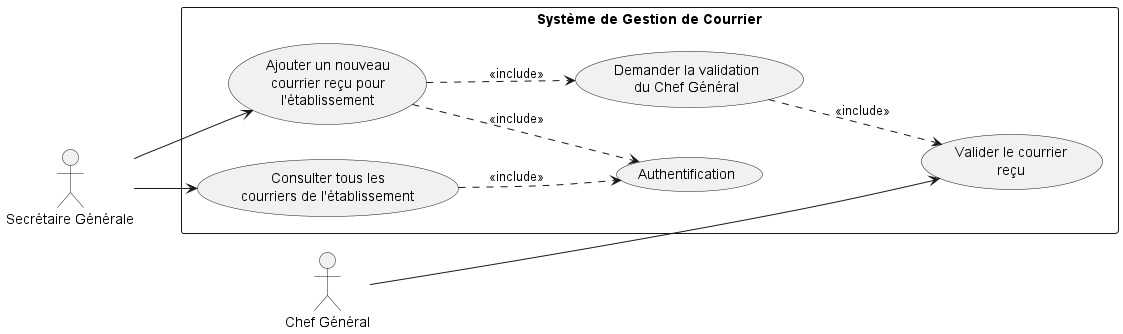
\includegraphics[width=14cm]{out/diagrams/usecases/puml/usecase_secretaire_general/usecase_secretaire_generale.png}
    \caption{Diagramme de cas d’utilisation de la secrétaire générale}
    \label{fig:cas_utilisation_secretaire_generale}
\end{figure}

\subsubsection{Diagramme de cas d’utilisation du chef d’organe}
\label{subsubsec:cas_utilisation_chef_organe}

\begin{figure}[H]
    \centering
    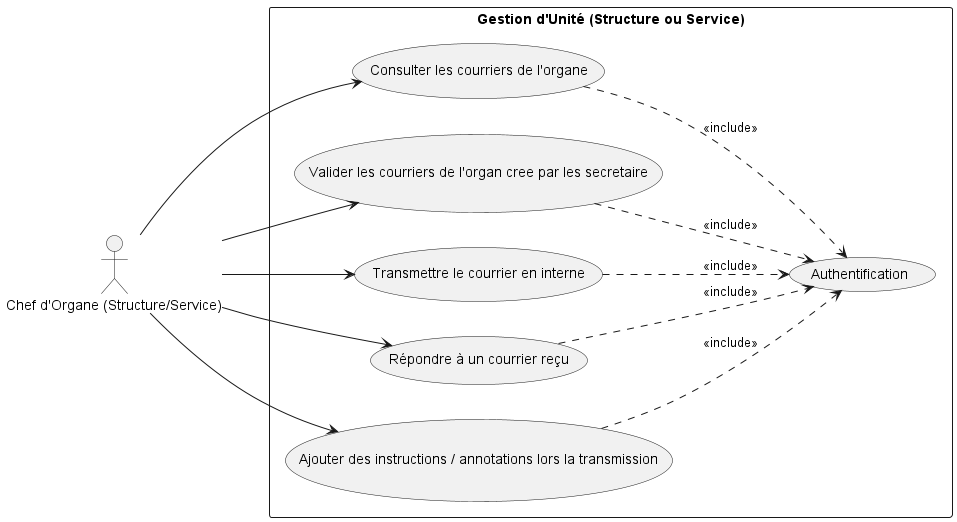
\includegraphics[width=14cm]{out/diagrams/usecases/puml/usecase_chef_organe/usecase_chef_organe.png}
    \caption{Diagramme de cas d’utilisation du chef d’organe}
    \label{fig:cas_utilisation_chef_organe}
\end{figure}
\subsubsection{Diagramme de cas d’utilisation de la secrétaire d’organe}
\label{subsubsec:cas_utilisation_secretaire_organe}

\begin{figure}[H]
    \centering
    
\includegraphics[width=14cm]{/mnt/c/Users/ENPEI/Desktop/courrier project/courier/out/diagrams/usecases/puml/usecase_secretaire/usecase_secretaire_organe.png}
    \caption{Diagramme de cas d’utilisation de la secrétaire d’organe}
    \label{fig:cas_utilisation_secretaire_organe}
\end{figure}
\subsubsection{Diagramme de cas d’utilisation de l’agent}
\label{subsubsec:cas_utilisation_agent}

\begin{figure}[H]
    \centering
    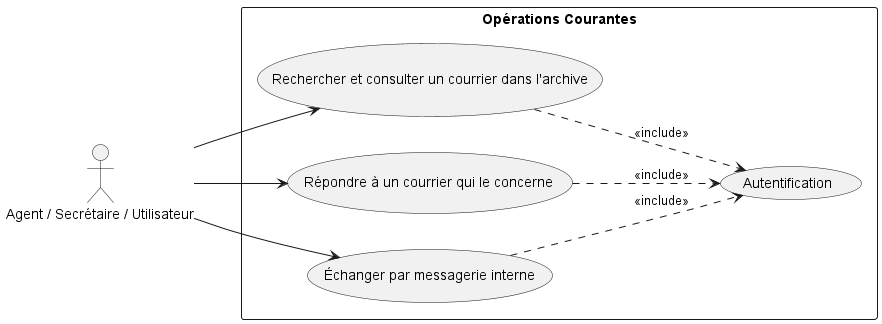
\includegraphics[width=14cm]{out/diagrams/usecases/puml/usecase_agent/usecase_agent.png}
    \caption{Diagramme de cas d’utilisation de l’agent}
    \label{fig:cas_utilisation_agent}
\end{figure}

\subsection{Diagrammes de séquence}
\label{subsec:diagrammes_sequence}

\subsubsection{Diagramme de séquence d’authentification}
\label{subsubsec:sequence_authentification}

\begin{figure}[H]
    \centering
    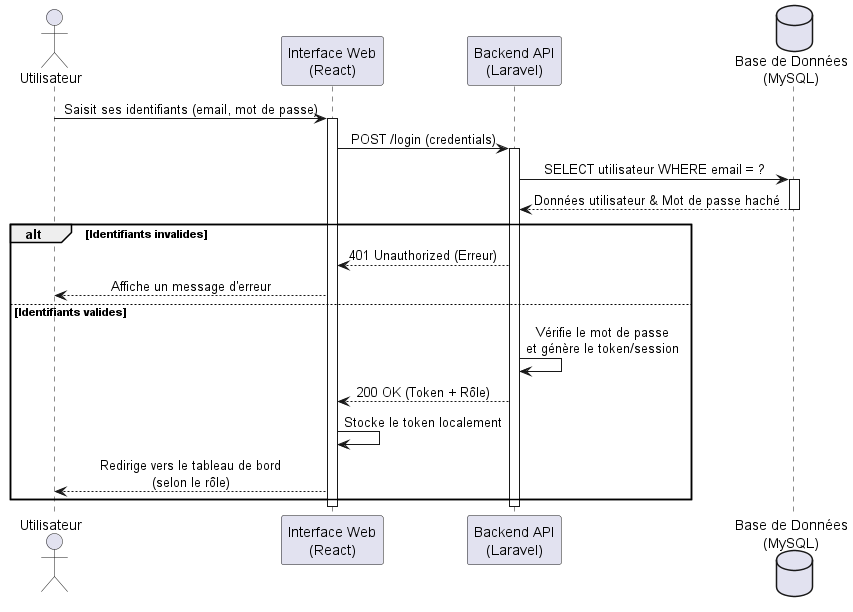
\includegraphics[width=14cm]{out/diagrams/seq_authentification/seq_authentification.png}
    \caption{Diagramme de séquence d’authentification}
    \label{fig:sequence_authentification}
\end{figure}

\subsubsection{Diagramme de séquence de création d’un courrier}
\label{subsubsec:sequence_creation_courrier}

\begin{figure}[H]
    \centering
    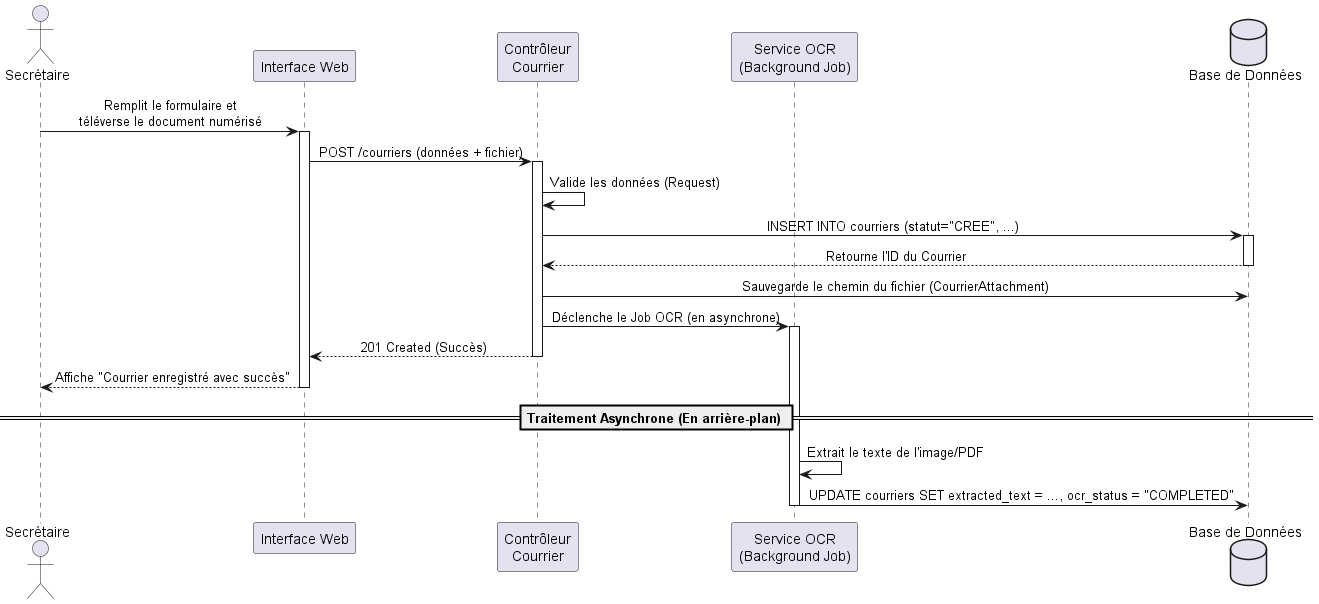
\includegraphics[width=14cm]{out/diagrams/seq_creation_courrier/seq_creation_courrier.png}
    \caption{Diagramme de séquence de création d’un courrier}
    \label{fig:sequence_creation_courrier}
\end{figure}

\subsubsection{Diagramme de séquence de transmission d’un courrier}
\label{subsubsec:sequence_transmission_courrier}

\begin{figure}[H]
    \centering
    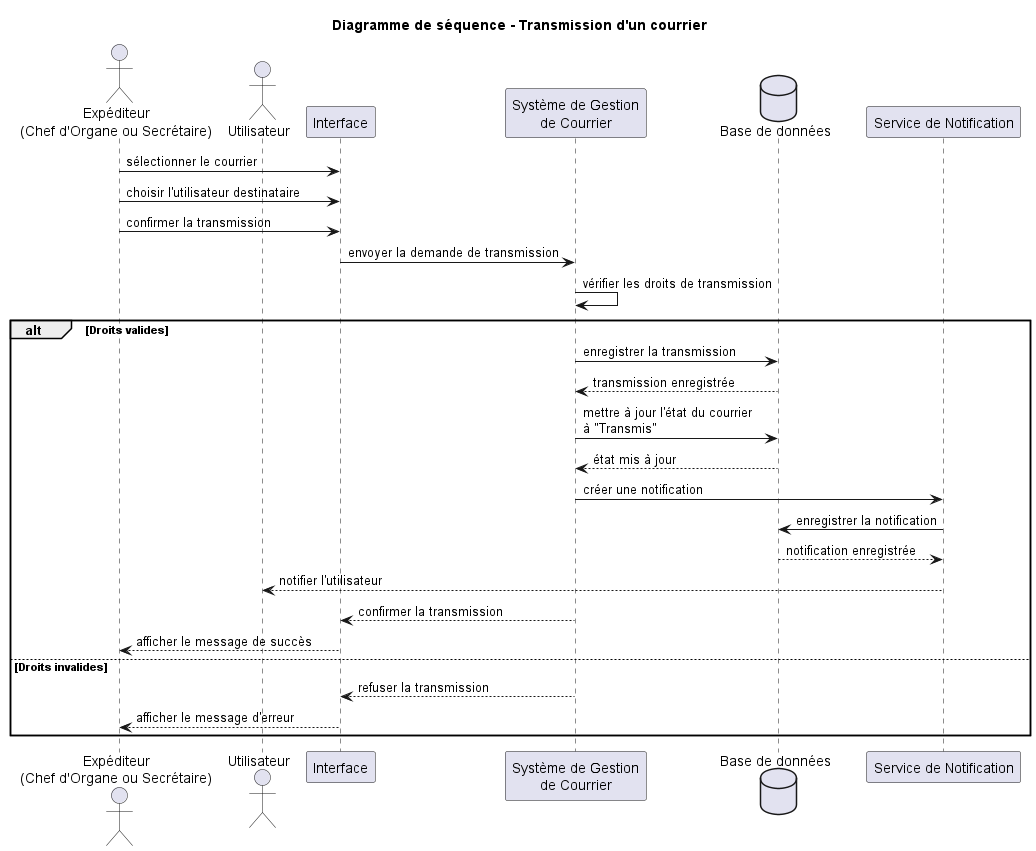
\includegraphics[width=14cm,height=0.5\textheight]{out/diagrams/seq_transmission_courrier/sequence_transmission_courrier.png}

    \caption{Diagramme de séquence de transmission d’un courrier}
    \label{fig:sequence_transmission_courrier}
\end{figure}

\subsubsection{Diagramme de séquence de réponse à un courrier}
\label{subsubsec:sequence_reponse_courrier}

\begin{figure}[H]
    \centering
    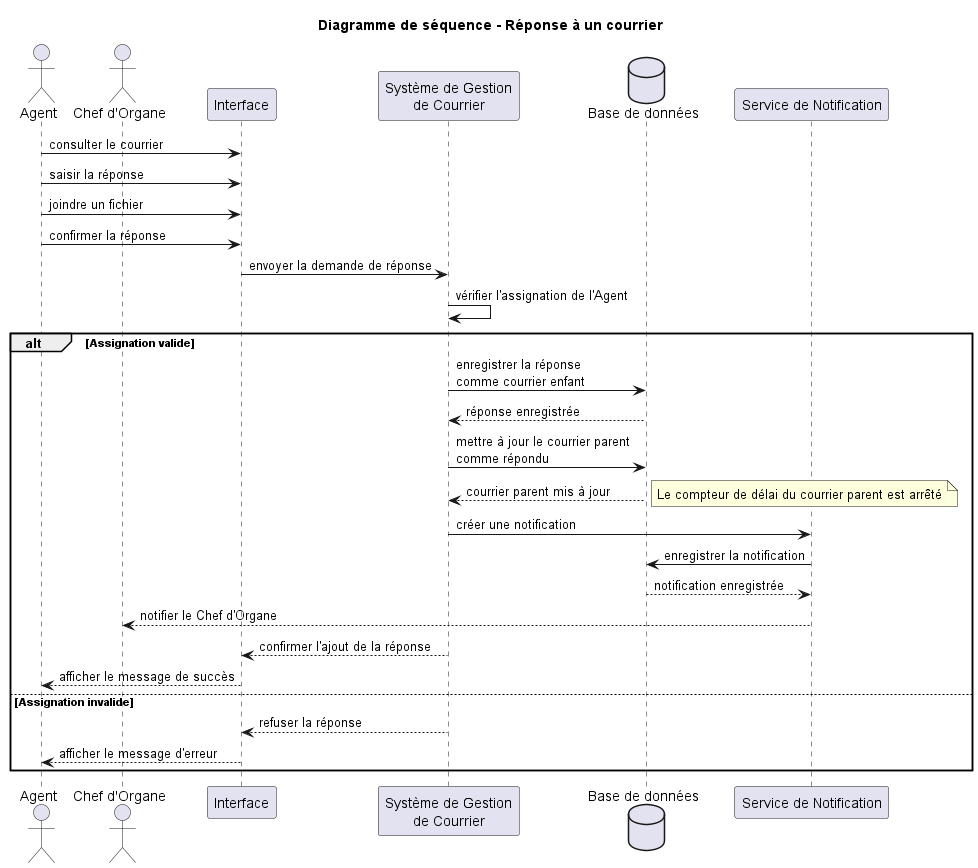
\includegraphics[width=14cm,height=0.3\textheight]{out/diagrams/seq_reponse_courrier/sequence_reponse_courrier.png}
    
    \caption{Diagramme de séquence de réponse à un courrier}
    \label{fig:sequence_reponse_courrier}
\end{figure}

\subsubsection{Diagramme de séquence d’archivage d’un courrier}
\label{subsubsec:sequence_archivage_courrier}

\begin{figure}[H]
    \centering
    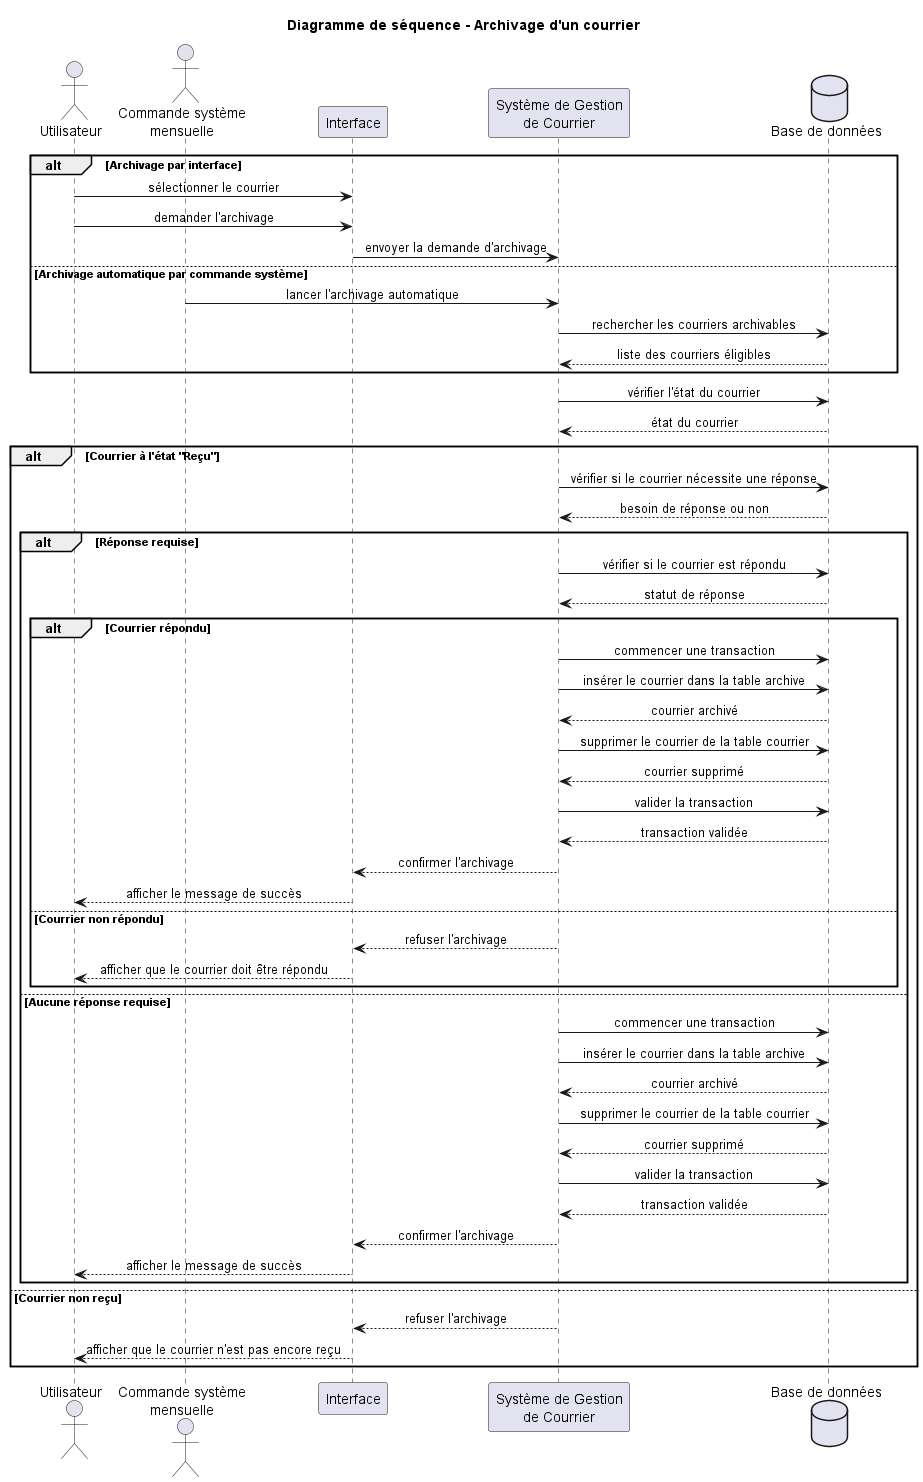
\includegraphics[width=0.90\textwidth,height=0.5\textheight]{out/diagrams/seq_archivage/sequence_archivage_courrier.png}
    \caption{Diagramme de séquence d’archivage d’un courrier}
    \label{fig:sequence_archivage_courrier}
\end{figure}

\subsubsection{Diagramme de séquence de recherche d’un courrier}
\label{subsubsec:sequence_recherche_courrier}

\begin{figure}[H]
    \centering
    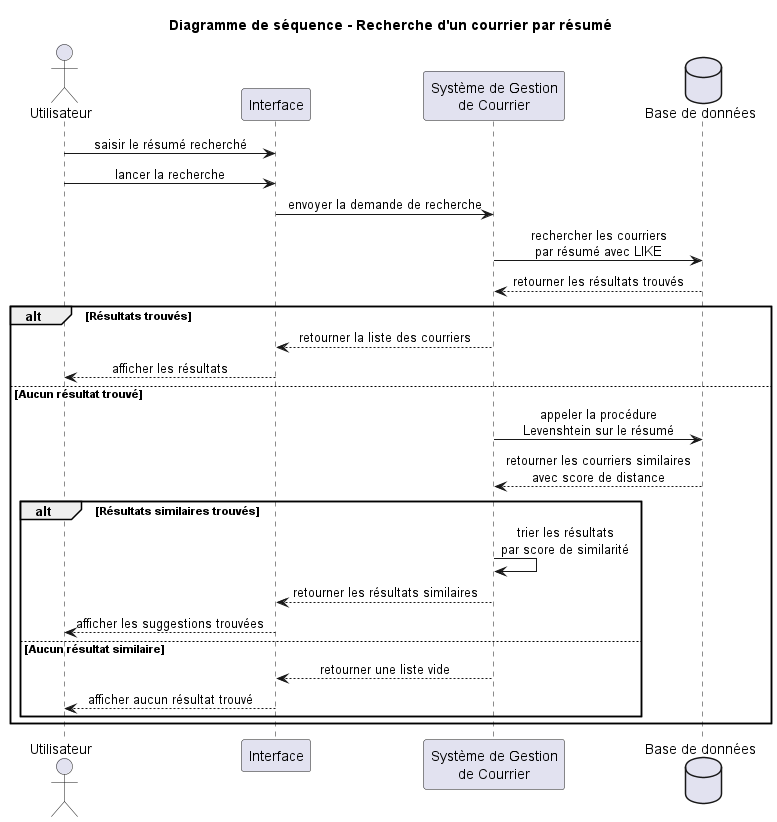
\includegraphics[width=0.90\textwidth,height=0.44\textheight]{out/diagrams/seq_recherche/sequence_recherche_courrier.png}
    \caption{Diagramme de séquence de recherche d’un courrier}
    \label{fig:sequence_recherche_courrier}
\end{figure}

\subsubsection{Diagramme de séquence de validation d’un courrier}
\label{subsubsec:sequence_validation_courrier}

\begin{figure}[H]
    \centering
    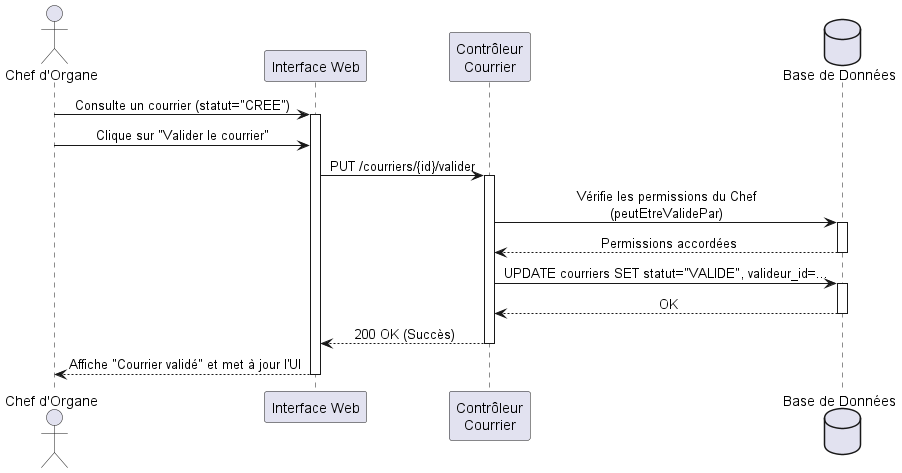
\includegraphics[width=14cm]{out/diagrams/seq_validation_courrier/seq_validation_courrier.png}
    \caption{Diagramme de séquence de validation d’un courrier}
    \label{fig:sequence_validation_courrier}
\end{figure}
\subsection{Diagramme d’états-transitions}
\label{subsec:diagramme_etats_transitions}

\begin{figure}[H]
    \centering
    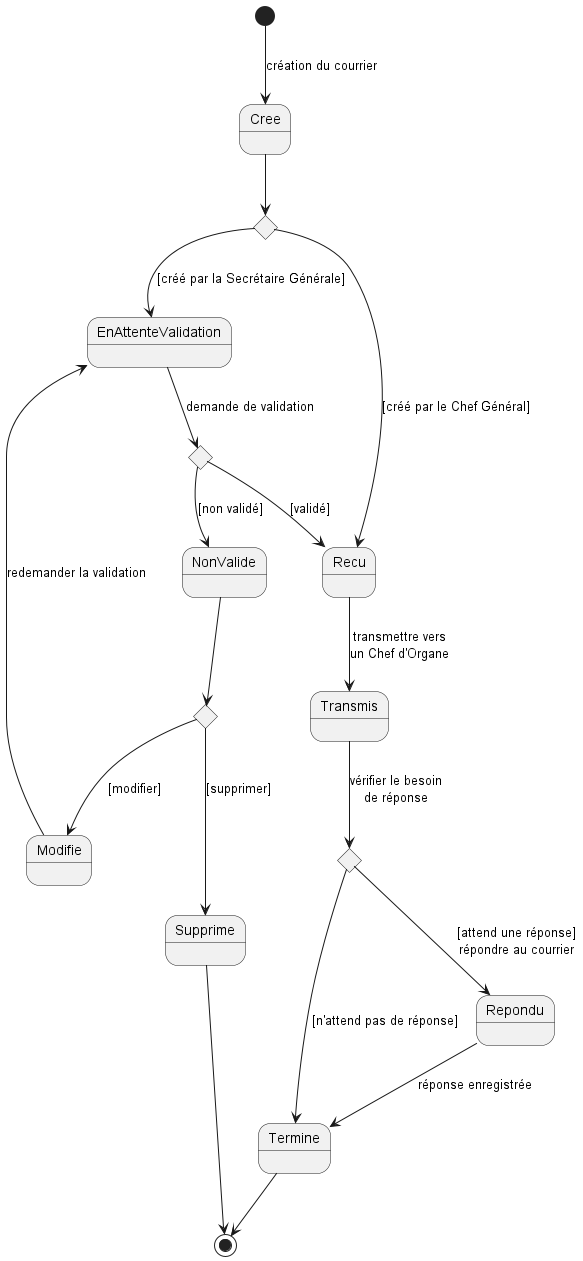
\includegraphics[width=\textwidth,height=0.85\textheight,keepaspectratio]{out/diagrams/usecases/puml/etat_courrier_creation_validation/etat_courrier.png}
    \caption{Diagramme d’états-transitions d’un courrier}
    \label{fig:etats_transitions_courrier}
\end{figure}